\documentclass{article}
\usepackage{graphicx}

\title{Automated testing analysis}
\author{Andrei Ionita}

\begin{document}
\maketitle

\section{Introduction and methodology}
This document provides the results and observations that I came across after using automated testing to test 
a MiniZinc model that uses dpath to find the shortest road between two given nodes, with additional mandatory vertex
constraints.


I implemented a python script to randomly generate numbers that would be used to make up a .dzn file, that would be used
as the input to the MiniZinc model. Afterwards, I created a bash script that would continuously run the python script and then
run the MiniZinc model on the provided, generated input. The limits I used for the bash script were the following:
\begin{enumerate}
    \item A single run of the model has an upper limit of 30 sec before it is terminated.
    \item The bash script repeats the process until 50 successful tests are generated.
\end{enumerate}
The output of the MiniZinc model was then appended to a different .txt file together with all the other results.
That file is what I used to analyse the model. Of course, the statistics are not based on only 50 successful runs of 
the model, 50 only representing the number that I chose as the size of a single batch of tests.

\section{Types of input and their respective statistics}
After a couple of tries using graphs with no more than 100 nodes and/or edges, and seeing that none of the inputs required
30 seconds of runtime, I decided to separate the testing and analysis into two parts: 
\begin{enumerate}
    \item Graphs with less than or equal to 100 nodes and edges(from this point onwards called small graphs).
    \item Graphs with more than 100 nodes/edges, and less than 1000 nodes and edges(from this point onwards called large graphs).
\end{enumerate}
The following sections will demonstrate my findings for both of these categories of inputs.


\subsection{Small Graphs}
Small note to begin with: The runtime for \textbf{all} of the tests was 0 ms. 

Given this observation, the only conclusions I can
draw are unrelated to time. An interesting and, at the same time, obvious finding is the fact that using \texttt{bounded\_path} 
instead of \texttt{bounded\_dpath} had a greater rate of success ('success' meaning that the model found a road that meets the constraints): 
$~40\%$ of the generated inputs had solutions for undirected graphs, while only around $25\%$ of generated inputs had solutions using the 
dpath algorithm. (directed graphs) Given the nature of directed and undirected graphs, this result was somewhat to be expected, since there 
overall, less roads between any two nodes in a directed graph than in an undirected one with the same edges. 

However, the disadvantage of using \texttt{bounded\_path} was the runtime itself. Compared to the 0 ms, instant runtime in the case of directed 
graphs, each run of the model took on average 7 seconds when using undirected graphs, most likely due to the sheer amount of possible roads. 
Therefore, automated testing was easier from the point of view of time spent in the case of the final algorithm - \texttt{bounded\_dpath}.

Below, I plotted 4 batches of tests, so 200 successful model runs. More specifically, the following figure shows the types of 
graphs generated by the python script. Even given the fact that the generation is entirely random, I thought the results can be interesting.

\begin{figure}[h]
    \centering 
    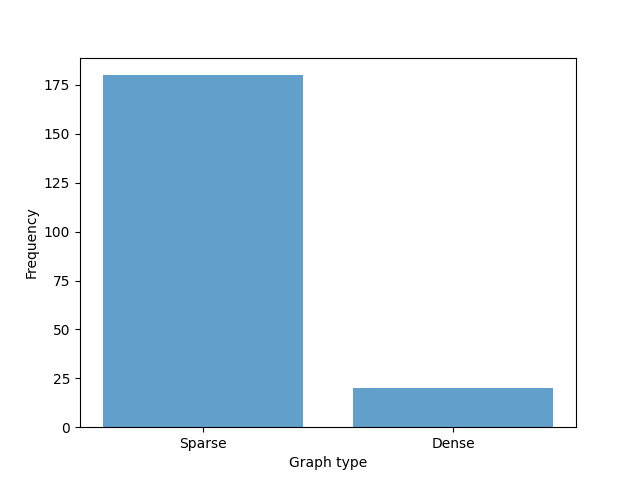
\includegraphics[width=0.8\linewidth]{../images/figure1.png}
    \caption{Figure showing distribution of graph types generated with a solution found by the model}
\end{figure}

To be precise, out of 200 random successful tests, 180 of them represent a sparse graph(less than half of possible edges), while only 20
of them represent dense graphs. While one would expect dense graphs to have a higher runtime, due to the low nature of the number of nodes 
and edges, as mentioned previously, the runtime was still always 0 ms. 
\subsection{Large Graphs} 
After playing around with small values (under 100) of edges and nodes, and seeing that the model had no problem 
finding a solution with respect to the constraints almost instantly, I decided to try testing the limits of the model's speed through higher values.

Initially, I wanted to try upping the upper limit of the number of edges and numbers to $10000$, but I quickly saw that the model really had trouble evaluating such a large input even with the runtime limit set to 60 seconds. 
So, after a long process of trial and error, the highest value I found actually feasible for the model was $1000$. The model did not manage to handle even inputs of 2000 nodes/edges in a reasonable amount 
of time(one minute).  

Therefore, with the new limits set, the time spent on the whole process of automated testing was expectedly longer than in the case of 'Small graphs'. 
A single batch of 50 successful tests took more than 500 tries (total tests - also including inputs without solution) and more than an hour overall. With this in mind, I decided 
to use 100 successful tests as the data sample for the upcoming analysis.

The first observation that needs to be mentioned is the fact that no dense graph was used as an input, due to the fact that the minimum number of nodes was 100 and the maximum number of edges of 
an input for the model was 1000. 

The next interesting idea that I was curious about was whether there was any correlation between the number of nodes/edges and the runtime of the model for 
a test. For each generated number of nodes and edges, I took the average of time spent and plotted the results. Using linear regression, I also plotted a line to be able to visualize any possible 
connection between the time and the no. of edges or nodes.

Inspecting \textit{Figure 2}, one can observe that there is no clear correlation between the number of nodes and the runtime(ignoring number of edges). There is a slight increase in time, but due to the small slope of the line, and 
the fact that the number of data samples with a high enough number of nodes is small, it can be argued that there is no conclusion to be drawn that would suggest that a higher number of nodes in a graph results in a higher runtime of 
the model.

On the other hand, the steeper slope that can be observed in \textit{Figure 3}, and the overall more balanced data points over the x-axis, seem to suggest 
a correlation between the number of edges and the runtime of the algorithm. This would also explain several failed experiments I tried, where I kept the number of nodes low, while increasing the number of edges when generating inputs. 


\begin{figure}[h]
    \centering 
    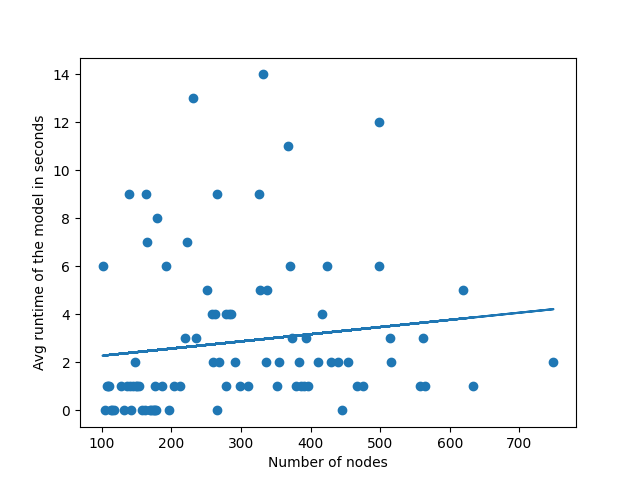
\includegraphics[width=0.8\linewidth]{../images/figure3.png}
    \caption{Scatter plot of showing the average runtime for the generated numbers of nodes, and a regression line fitted to the data}
\end{figure}

\begin{figure}[h]
    \centering 
    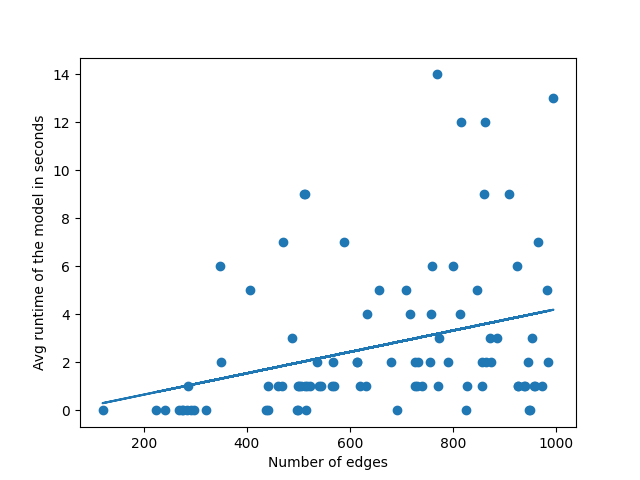
\includegraphics[width=0.8\linewidth]{../images/figure2.png}
    \caption{Scatter plot of the average runtime/number of edges, and a regression line fitted to the data}
\end{figure}


\end{document} 